\documentclass[tikz,border=3.14mm]{standalone}
\usetikzlibrary{positioning}
\newcommand{\blok}[4]{%
	\def\sft{2pt} % shift from border of cells to coloured rectangles
	\draw[rounded corners=2pt,opacity=0.8,#1,fill=#1!50,thick] ([shift={(\sft,-\sft)}]#2.north west) rectangle ([shift={(-\sft,\sft)}]#3.south east);
	\node[right] at ([xshift=-0.44*\s cm]#2.center) {#4};
}
\begin{document}
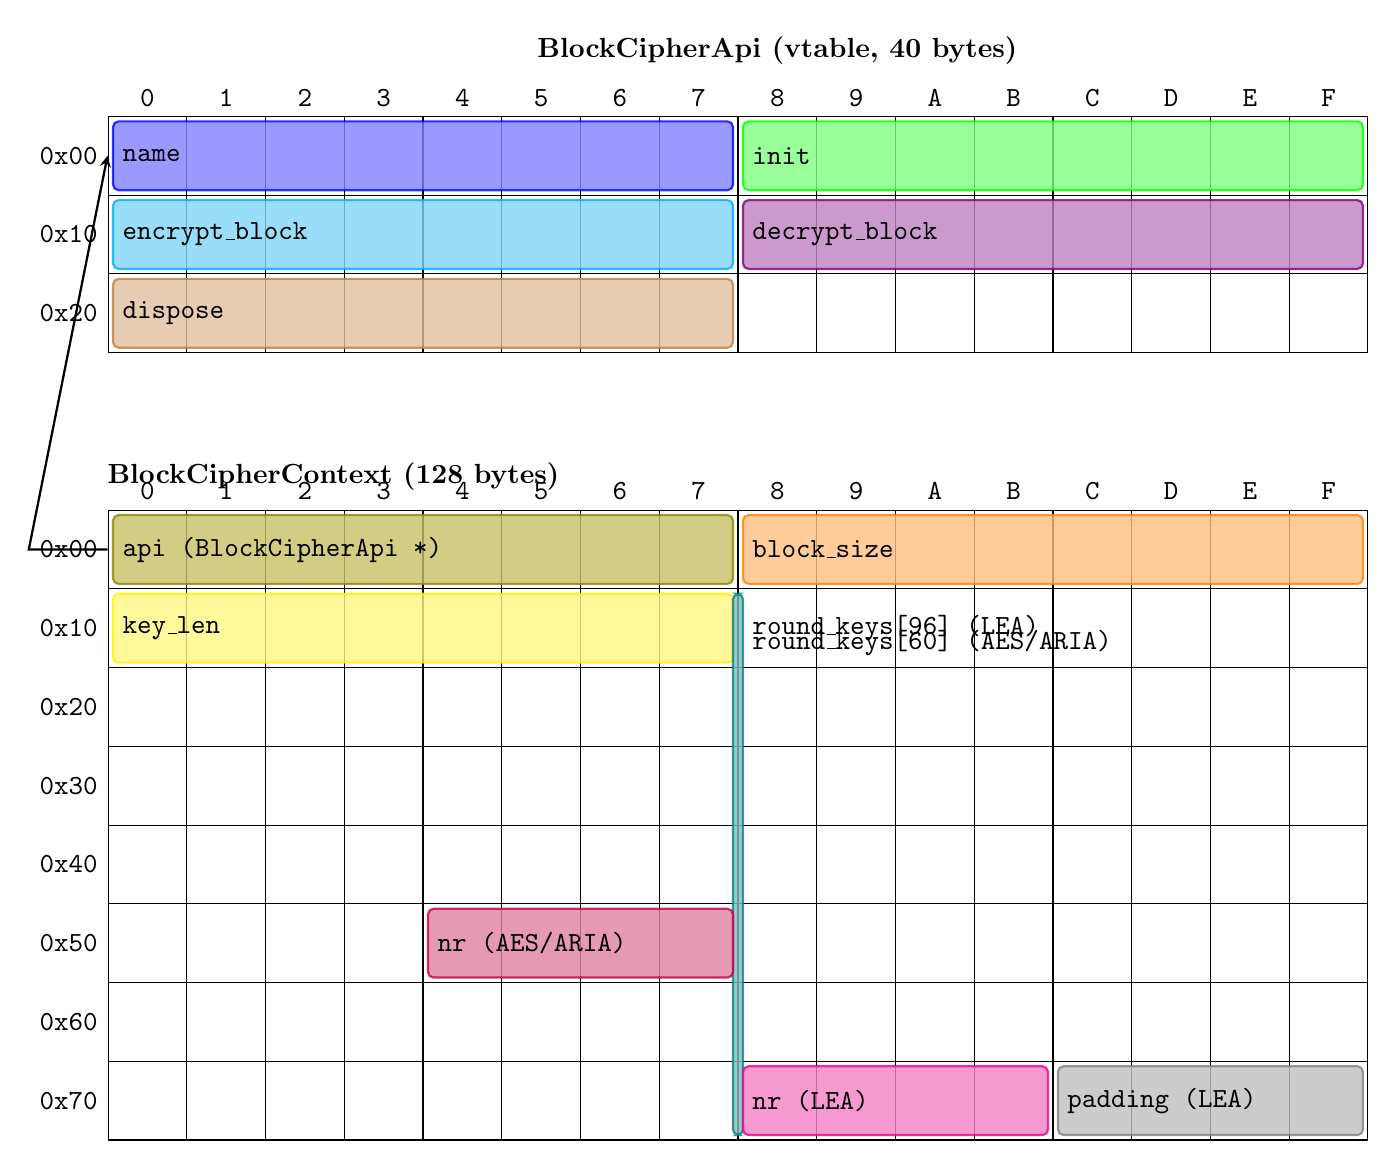
\begin{tikzpicture}[font=\ttfamily]
	\def\s{1} % cell size in cm
	
	%--- BlockCipherContext memory grid (8 rows x 16 cols = 128 bytes) ---
	\foreach \l [count=\k from 0] in {a,...,h}{% rows a-h
		\foreach \i in {0,...,15}{% cols 0-F
			\node[draw, minimum size=\s cm] (\l\i) at (\i*\s, -\k*\s) {};}
	}
	% Row/column labels for context
	\foreach \c [count=\i from 0] in {0,...,9,A,B,...,F}{
		\node[above] at (a\i.north) {\texttt{\c}};}
	\foreach \l [count=\i from 0] in {a,...,h}{
		\node[left] at (\l0.west) {\texttt{0x\i0}};}
	% Label the entire context structure
	\node[above left=5pt of a0.north west, anchor=south west, font=\bfseries] {BlockCipherContext (128 bytes)};
	
	\begin{scope}[yshift=5cm, xshift=-18cm]
	%--- BlockCipherApi vtable memory grid (3 rows x 16 cols = 48 bytes, 40 used) ---
	\foreach \l [count=\k from 0] in {i,...,k}{% rows i-k
		\foreach \i in {0,...,15}{% cols 0-F
			\node[draw, minimum size=\s cm] (\l\i) at (\i*\s + 18*\s, -\k*\s) {};}
	}
	% Row/column labels for vtable
	\foreach \c [count=\i from 0] in {0,...,9,A,B,...,F}{
		\node[above] at (i\i.north) {\texttt{\c}};}
	\foreach \l [count=\i from 0] in {i,...,k}{
		\node[left] at (\l0.west) {\texttt{0x\i0}};}
	% Label the entire vtable structure
	\node[above=15pt of i8.north, anchor=south, font=\bfseries] {BlockCipherApi (vtable, 40 bytes)};
	\end{scope}
	
	%--- Highlight BlockCipherContext fields (using \blok) ---
	%api pointer (8 bytes)
	\blok{olive}{a0}{a7}{api (BlockCipherApi *)}
	% block_size (size_t, 8 bytes)
	\blok{orange}{a8}{a15}{block\_size}
	% key_len (size_t, 8 bytes)
	\blok{yellow}{b0}{b7}{key\_len}
	% round_keys[96] for LEA (largest union member, 96 bytes)
	\blok{teal}{b8}{h7}{round\_keys[96] (LEA)}
	% round_keys[60] for AES/ARIA (60 bytes) – draw without label to avoid overlap, label manually below
%	\blok{red}{b8}{f3}{}
%	% nr for AES/ARIA (int, 4 bytes at 0x54–0x57)
	\blok{purple}{f4}{f7}{nr (AES/ARIA)}
%	% nr for LEA (int, 4 bytes at 0x78–0x7B)
	\blok{magenta}{h8}{h11}{nr (LEA)}
%	% padding (4 bytes at 0x7C–0x7F, only in LEA struct)
	\blok{gray}{h12}{h15}{padding (LEA)}
	
	% Manual label for AES/ARIA round_keys (60 bytes)
	\node[right] at ([xshift=-0.44*\s cm, yshift=-1.2ex] b8.center) {\texttt{round\_keys[60] (AES/ARIA)}};
	
	%--- Highlight BlockCipherApi (vtable) fields ---
	% name pointer (8 bytes)
	\blok{blue}{i0}{i7}{name}
	% init function pointer (8 bytes)
	\blok{green}{i8}{i15}{init}
	% encrypt_block function pointer (8 bytes)
	\blok{cyan}{j0}{j7}{encrypt\_block}
	% decrypt_block function pointer (8 bytes)
	\blok{violet}{j8}{j15}{decrypt\_block}
	% dispose function pointer (8 bytes)
	\blok{brown}{k0}{k7}{dispose}
	
	%--- Pointer arrows linking to targets ---
	% api pointer -> start of vtable
	\draw[->, >=stealth, thick] (a0.west) -- ++(-1,0) -- (i0.west);
%	% Function pointers -> AES functions
%	\node[anchor=west] (NameStr) at ([xshift=2cm, yshift=+5pt] i7.east) {\texttt{"AES"}};
%	\draw[->, >=stealth, thick] (i7.east) -- (NameStr.west);
%	\node[anchor=west] (InitFn) at ([xshift=2cm, yshift=-5pt] i15.east) {\texttt{aes\_init}};
%	\draw[->, >=stealth, thick] (i15.east) -- (InitFn.west);
%	\node[anchor=west] (EncryptFn) at ([xshift=2cm, yshift=+5pt] j7.east) {\texttt{aes\_encrypt}};
%	\draw[->, >=stealth, thick] (j7.east) -- (EncryptFn.west);
%	\node[anchor=west] (DecryptFn) at ([xshift=2cm, yshift=-5pt] j15.east) {\texttt{aes\_decrypt}};
%	\draw[->, >=stealth, thick] (j15.east) -- (DecryptFn.west);
%	\node[anchor=west] (DisposeFn) at ([xshift=2cm] k7.east) {\texttt{aes\_dispose}};
%	\draw[->, >=stealth, thick] (k7.east) -- (DisposeFn.west);
\end{tikzpicture}
\end{document}
